\section{Buscas}
\begin{frame}

    \frametitle{Buscas}

   \begin{block}{}
     \begin{itemize}
      \item Requisito: conceitos de listas e recursividade  dominados!
       \pause
      \item Além destes: conceitos grafos, árvores de busca, nós, etc
         
       \pause
      \item Pois, problemas em geral
      se apresentam como uma conexão complexa tipo um \textit{grafo},
      e a varredura sob este grafo é sistemática
      sob uma \textit{árvore de busca}
      \pause
      
     \item Então, computar listas em Picat, é a nossa estratégia
     de resolver problemas!

    \end{itemize}
    
    \end{block}
    
\end{frame}



\begin{frame}[fragile, allowframebreaks=0.9]
  \frametitle{Ciclo Euleriano}

\begin{figure}[!htb]
\centering
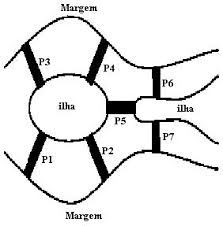
\includegraphics[width=0.60\textwidth, height=0.650\textheight]{figures/ilhas_euler.jpeg}
%%%prolog/scale=0.47
%\label{fig_nos_estados}
\caption{Ciclo Euleriano -- Problema das Pontes de Königsberg}
\end{figure}


\framebreak

\begin{itemize}
  \item No século 18 havia na cidade de Königsberg (antiga Prússia)  um conjunto de sete pontes
 (identificadas pelas letras de P1 até P7 na figura ao lado ) que cruzavam o rio  Prególia. 
 Elas conectavam duas ilhas  entre si e as ilhas com as margens esquerda
 e direita.
 
\item Os habitantes daquela cidade perguntavam-se se era possível cruzar 
as sete pontes numa caminhada contínua sem que se passasse duas vezes por 
qualquer uma das pontes.

\item  Embora intrigante, este problema foi atacado por Leonard Euler (1736) e demonstrou
que isto não era possível para um grafo qualquer

\item Curiosamente, este problema, computacionalmente é \underline{\textit{fácil}} de resolver!
\end{itemize}

\end{frame}



\begin{frame}[fragile, allowframebreaks=0.9]
  \frametitle{Caminho Hamiltoniano}


\begin{figure}[!htb]
\centering
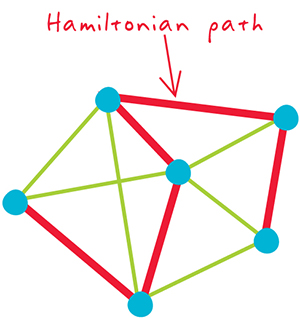
\includegraphics[width=.6\textwidth, height=0.60\textheight]{figures/hamiltonian_path.jpg}
%%%prolog/scale=0.47
%\label{fig_nos_estados}
\caption{Caminho Hamiltoniano -- Há um caminho que passe por todas cidades uma única vez?}
\end{figure}


\framebreak

\begin{itemize}
  \item Diferente do ciclo Euleriano, o caminho Hamiltoniano, origem
  e destino são diferentes
 
\item Todos os nós precisam ser visitados uma única vez sem repetição

\item  Num grafo pode haver muitos caminhos  Hamiltonianos, mas, pode
       não existir nenhum!

\item Ao contrário do ciclo Euleriano, este problema, computacionalmente é \underline{\textit{difícil}} de resolver!

\item Mas é este que vamos usar como exemplo, com um algoritmo  ingênuo.
\end{itemize}

\end{frame}


\begin{frame}[fragile,  allowframebreaks=0.8]
\frametitle{Problemas, Estados, Grafos e  Árvores de Buscas}

Contextualizando estes termos:

\begin{itemize}

  \item Em geral, problemas podem ser vistos como \textit{fotografias 
  instantâneas} de uma situação, isto é, \textbf{um estado discreto}
   
  \item Uma \textit{sucessão} destes estados, compõem \textit{um caminho} de um estado $i$ ao estado $j$
  
  \item Assim, estes \textit{estados} são representados pelos \textit{nós dos grafos}, e a ligação entre 
  estes, são resultados de \textit{uma ação}, mudança ou evolução do problema
  
  \item Há um estado particular chamado \textit{inicial},  vários outros de estados \textit{intermediários},
   e outros estados \textit{finais}
  
  \item Se o problema tiver várias soluções,  o mesmo apresenta vários caminhos do estado inicial ao  final.
  
  \item Assim uma sucessão ou transição válida entre estados, é conhecido como uma \textit{solução} ou \textit{prova}
     do problema

  \item Essencialmente vamos varrer uma estrutura
     entre estados ou nós, de modo sistemático até encontrarmos
     uma solução aceitável/desejável.

    \item Logo, vamos empregar alguns conceitos da teoria dos grafos, em modelar problemas e resolvê-los 
  por um esquema de busca computacional
  
    
\end{itemize}

\end{frame}


%%%%%%%%%%%%%%

\begin{frame}[fragile]
\frametitle{Problemas de Grafos se Transformam em Árvores de Buscas}

\begin{figure}[!htb]
\centering
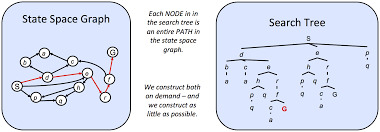
\includegraphics[width=.99\textwidth, height=0.55\textheight]{figures/espaco-estado-arvore.jpg}
%%%prolog/scale=0.47
%\label{fig_nos_estados}
\caption{Google ...}
\end{figure}

\textcolor{red}{Resumindo, os problemas são modelados  em 
estruturas  complexas, tais como grafos, mas o processo de solução
se mantém: realizar uma busca, tal como uma estrutura de uma árvore }

\end{frame}




\begin{frame}[fragile, allowframebreaks=0.9]
  \frametitle{Núcleo Geral de Buscas}



\textcolor{red}{Pseudo-código já em Picat}

\begin{verbatim}
resolve(P) =>
      inicio(Start),
      busca(Start,[Start],Qsol),
      imprime_saida(Qsol,P).

busca(S,P,P) ?=>  objetivo(S).    % objetivo alcancado : FIM    
busca(S,Visited,P) =>
     proximo_estado(S,Nxt),       % gera um proximo estado  
     estado_seguro(Nxt),          % verifica se este estado é válido 
     sem_loop(Nxt,Visited),       % verifica se está em loop .. repete estados 
     busca(Nxt,[Nxt|Visited],P).  % continue a busca recursiva 
\end{verbatim}


\framebreak


\begin{verbatim}

sem_loop(Nxt,Visited) :-
      \+member(Nxt,Visited).

proximo_estado(S,Nxt) =>   < fill in here >.
estado_seguro(Nxt) =>     < fill in here >.
sem_loop(Nxt,Visited) =>  < fill in here >.     
                       
inicio(...).
objetivo(...).

\end{verbatim}


\textcolor{red}{Vamos reescrever este pseudo-código em um problema!}


\end{frame}


\begin{frame}[fragile]
\frametitle{Caminho Hamiltoniano Aplicado}

\begin{figure}[!htb]
\centering
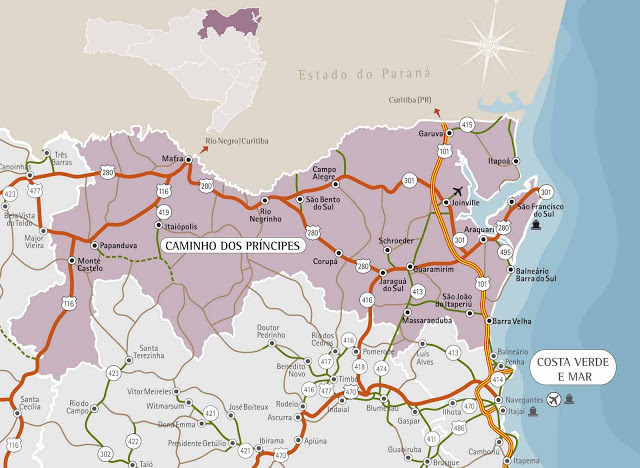
\includegraphics[width=.8\textwidth, height=0.567\textheight]{figures/mapa-norte-santa-catarina.jpg}
%%%prolog/scale=0.47
%\label{fig_nos_estados}
%\caption{Mapa do norte de Santa Catarina}
\end{figure}

Seja um viajante que sai cedo de Joinville, e chegar a noite
em Blumenau, passando por algumas destas cidades uma única vez!

\end{frame}


\begin{frame}[fragile]
\frametitle{Cidades Escolhidas pelo Viajante}

\begin{figure}[!htb]
\centering
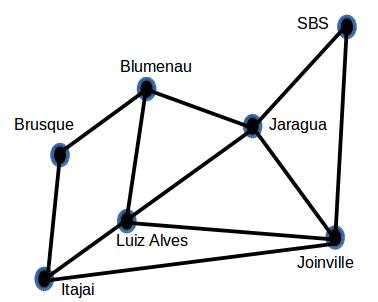
\includegraphics[width=.8\textwidth, height=0.567\textheight]{figures/mapa01SC.jpg}
%%%prolog/scale=0.47
%\label{fig_nos_estados}
%\caption{Mapa do norte de Santa Catarina}
\end{figure}

\end{frame}




\begin{frame}[fragile, allowframebreaks=0.9]
 \frametitle{\textit{O nosso viajante}}

\begin{itemize}
  \item Em nosso problema temos 7 cidades pré-escolhidas

  \item A lista de cidades são:
  \begin{verbatim}
index(-) %% lista de todas cidade do mapa
as_cidades( [ brusque, blumenau, itajai, luiz_alves,
            jaragua, sao_bento, joinville ] ).
\end{verbatim}

  \item  Duas cidades em particular
\begin{verbatim}
index(-)
destino( blumenau ).

index(-)
origem( joinville ).
\end{verbatim}  

  
\item As estradas transitáveis entre as cidades definem
  o nosso mapa, consequentemente um grafo entre
  cidades:
\begin{verbatim}
%% MAPA da região
index(-,-)
arco(joinville, sao_bento)  .
arco(joinville, itajai)     .
arco(joinville, jaragua)     .
arco(joinville, luiz_alves)     .
arco(jaragua, sao_bento)    .
arco(jaragua, blumenau)     .
arco(jaragua, luiz_alves)   .
arco(itajai, luiz_alves)    . 
arco(blumenau, luiz_alves)    . 
arco(blumenau, itajai)      .
arco(brusque, itajai)       .
arco(brusque, blumenau)     .
\end{verbatim} 
  
\item Claro, este problema é pequeno e construindo o grafo dá para perceber que existe
algumas soluções

  \item Para resolver este problema vamos utilizar uma \textit{busca em profundidade}
  
  \item Esta \textit{busca em profundidade}, encontra-se inserida no contexto buscas em geral,
  visto anteriormente
\end{itemize}


\end{frame}




\begin{frame}[fragile]
 \frametitle{O código}

\begin{itemize}
  \item Acompanhar as explicações do código de:\\
\url{https://github.com/claudiosa/CCS/blob/master/picat/hamiltoniano_DFS.pi}

  \item Confira a execuç\~ao
\end{itemize}
\end{frame}



\begin{frame}[fragile]
\frametitle{Uma Soluç\~ao}

\begin{figure}[!htb]
\centering
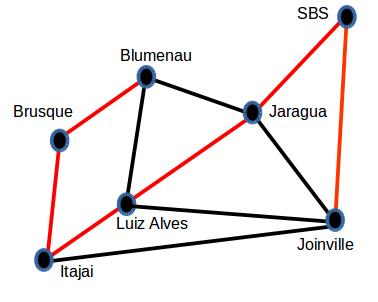
\includegraphics[width=.8\textwidth, height=0.567\textheight]{figures/mapa02SC.jpg}
%%%prolog/scale=0.47
%\label{fig_nos_estados}
%\caption{Mapa do norte de Santa Catarina}
\end{figure}

\end{frame}









